\documentclass[12pt,a4paperpaper,authoryear]{elsarticle} %review=doublespace preprint=single 5p=2 column
%%% Begin My package additions %%%%%%%%%%%%%%%%%%%
\usepackage[hyphens]{url}
\usepackage{lineno} % add
\usepackage{setspace}
\onehalfspacing

\usepackage{mathpazo}

\providecommand{\tightlist}{%
  \setlength{\itemsep}{0pt}\setlength{\parskip}{0pt}}

\biboptions{sort&compress} % For natbib
\usepackage{graphicx}
\usepackage{booktabs} % book-quality tables
%% Redefines the elsarticle footer
%\makeatletter
%\def\ps@pprintTitle{%
% \let\@oddhead\@empty
% \let\@evenhead\@empty
% \def\@oddfoot{\it \hfill\today}%
% \let\@evenfoot\@oddfoot}
%\makeatother

% A modified page layout
\textwidth 6.75in
\oddsidemargin -0.15in
\evensidemargin -0.15in
\textheight 9in
\topmargin -0.5in
%%%%%%%%%%%%%%%% end my additions to header

\usepackage[T1]{fontenc}
\usepackage{amssymb,amsmath}
\usepackage{ifxetex,ifluatex}
\usepackage{fixltx2e} % provides \textsubscript
% use upquote if available, for straight quotes in verbatim environments
\IfFileExists{upquote.sty}{\usepackage{upquote}}{}
\ifnum 0\ifxetex 1\fi\ifluatex 1\fi=0 % if pdftex
  \usepackage[utf8]{inputenc}
\else % if luatex or xelatex
  \usepackage{fontspec}
  \ifxetex
    \usepackage{xltxtra,xunicode}
  \fi
  \defaultfontfeatures{Mapping=tex-text,Scale=MatchLowercase}
  \newcommand{\euro}{€}
\fi
% use microtype if available
\IfFileExists{microtype.sty}{\usepackage{microtype}}{}
\usepackage[margin=1in]{geometry}
\usepackage{natbib}
\bibliographystyle{model5-names}
\usepackage{longtable}
\usepackage{graphicx}
% We will generate all images so they have a width \maxwidth. This means
% that they will get their normal width if they fit onto the page, but
% are scaled down if they would overflow the margins.
\makeatletter
\def\maxwidth{\ifdim\Gin@nat@width>\linewidth\linewidth
\else\Gin@nat@width\fi}
\makeatother
\let\Oldincludegraphics\includegraphics
\renewcommand{\includegraphics}[1]{\Oldincludegraphics[width=\maxwidth]{#1}}
\ifxetex
  \usepackage[setpagesize=false, % page size defined by xetex
              unicode=false, % unicode breaks when used with xetex
              xetex]{hyperref}
\else
  \usepackage[unicode=true, colorlinks]{hyperref}
\fi
\setlength{\parindent}{0pt}
\setlength{\parskip}{6pt plus 2pt minus 1pt}
\setlength{\emergencystretch}{3em}  % prevent overfull lines
\setcounter{secnumdepth}{0}
% Pandoc toggle for numbering sections (defaults to be off)
\setcounter{secnumdepth}{0}
% Pandoc header


\usepackage[nomarkers]{endfloat}

%% My customizations %%%%%%%%
%% Loading Packages
\usepackage[inline]{enumitem}
\usepackage{float}
\usepackage{xfrac}
\usepackage{tabularx}
\usepackage{tabularx}
\usepackage[dvipsnames]{xcolor}
\usepackage{pgf, tikz}
\usepackage{amsthm}
\newtheorem{mydef}{Definition}

%% Custom macros
\newcommand{\bs}[1]{\ensuremath{\boldsymbol{#1}}}
\newcommand{\diag}[1]{\mathrm{diag}\left(#1\right)}
\newcommand{\seq}[3][1]{\ensuremath{#2_{#1},\ldots,\,#2_{#3}}}
\newcommand{\note}[1]{\marginpar{\scriptsize\tt{\color{RoyalBlue}#1}}}
\newcommand{\edit}[1]{{\color{OrangeRed} #1}}

%% Custom Lengths
\setlength{\parindent}{0pt}
\setlength{\parskip}{9pt}

%% Define Colors
\newcommand\myshade{85}
\colorlet{mylinkcolor}{violet}
\colorlet{mycitecolor}{YellowOrange}
\colorlet{myurlcolor}{Aquamarine}

%% Hyperlink Setup
\AtBeginDocument{%
  \hypersetup{breaklinks=true,
              bookmarks=true,
              pdfauthor={},
              pdftitle={simrel-m -- A versatile tool for data simulation for multi-response linear model data based on the concept of relevant subspace of predictor space},
              colorlinks=true,
              urlcolor=myurlcolor!\myshade!black,
              linkcolor=mylinkcolor!\myshade!black,
              citecolor=mycitecolor!\myshade!black,
              pdfborder={0 0 0}}
}
% \urlstyle{same}  % don't use monospace font for urls
% 
%% End my customizations %%%%%%%%%

\begin{document}
\begin{frontmatter}

  \title{simrel-m -- A versatile tool for data simulation for multi-response
linear model data based on the concept of relevant subspace of predictor
space}
    \author[Norwegian University of Life Sciences]{Raju Rimal}
  
  
    \author[Norwegian University of Life Sciences]{Trygve Almøy}
  
  
    \author[Norwegian University of Life Sciences]{Solve Sæbø\corref{c1}}
  
   \cortext[c1]{Dep. of Chemistry and Food Science, NMBU, Ås
(\href{http://nmbu.no}{nmbu.no})}
    
  \begin{abstract}
  \small
  Data science is generating enormous amounts of data, and new and
  advanced analytical methods are constantly being developed to cope with
  the challenge of extracting information from such ``big-data''.
  Researchers often use simulated data to assess and document the
  properties of these new methods, and in this paper we present
  \texttt{simrel-m}, which is a versatile and transparent tool for
  simulating linear model data with extensive range of adjustable
  properties. The method is based on the concept of relevant components
  \citet{helland1994comparison}, which is equivalent to the envelope model
  \citet{cook2013envelopes}. It is a multi-response extension of
  \texttt{simrel} \citet{saebo2015simrel}, and as \texttt{simrel} the new
  approach is essentially based on random rotations of latent relevant
  components to obtain a predictor matrix \(\mathbf{X}\), but in addition
  we introduce random rotations of latent components spanning a response
  space in order to obtain a multivariate response matrix \(\mathbf{Y}\).
  The properties of the linear relation between \(\mathbf{X}\) and
  \(\mathbf{Y}\) are defined by a small set of input parameters which
  allow versatile and adjustable simulations. Sub-space rotations also
  allow for generating data suitable for testing variable selection
  methods in multi-response settings. The method is implemented as an
  R-package which serves as an extension of the existing \texttt{simrel}
  packages \citet{saebo2015simrel}.
  \end{abstract}
   \begin{keyword} \footnotesize \texttt{simrel-2.0}, \texttt{simrel} package in r, data
simulation, linear model, \texttt{simrel-m} \sep \end{keyword}
 \end{frontmatter}

\section*{Preface}\label{preface}
\addcontentsline{toc}{section}{Preface}

\section{Introduction}\label{introduction}

\emph{General aspects}

Technological advancement has opened a door for complex and
sophisticated scientific experiments that was not possible before. Due
to this change, enormous amounts of raw data are generated which
contains massive information but difficult to excavate. Finding
information and performing scientific research on these raw data is now
becoming another problem. In order to tackle this situation new methods
are being developed. However, before implementing any methods, it is
essential to test its performance. Often, researchers use simulated data
for the purpose which itself is a time-consuming process. The main focus
of this paper is to present a simulation method, along with an r-package
called \texttt{simrel-m}, that is versatile in nature and yet simple to
use.

The method is based on principal of relevant space for prediction which
assumes that there exists a subspace in the complete space of responses
that is spanned by a subset of eigenvectors of predictor variables. The
method and the r-package based on this principle not only has ability to
simulate wide range of multi-response linear model data but also let
researcher to specify which components of predictors \((\mathbf{X})\)
are relevant for a component of responses \(\mathbf{Y}\). This enables
the possibility to construct data for evaluating methods developed for
variable selection.

A vast literature on simulation is present but most of them are
developed to address the specific problems their study was dealing with.
\citet{saebo2015simrel} has presented a generic tool that is capable of
simulating linear model data as an r-package \texttt{simrel}. This paper
extends the methods to simulate multivariate response.

\emph{Application of \texttt{simrel-m}}

The simple interface of \texttt{simrel-m} for sophisticated simulation
opens for numerous applications in various disciplines among which some
of them are discussed below.

\begin{description}
\tightlist
\item[\emph{Educational Purpose:}]
Explaining multivariate statistics and edify people is a difficult and
strategic task. Instructors spend lots of time just to find suitable
datasets for explaining some issue. For instance --
\item[\emph{Model and methods testing:}]
Imagine a situation where a researcher is collecting enormous amount of
data which takes both time and money. Before going into extensive
sampling, a pilot project is started and samples were collected using
various techniques. Each of them are modelled with different estimation
methods. The researcher would like to compare the sampling methods or
estimation procedures that will the suitable for the final project. A
simulated dataset based on the pilot project may help to identify the
most appropriate sampling methods or estimation procedures.
\item[\emph{Understanding and developing multivariate statistics:}]
New estimation methods are being developed to address mordern and
complicated situations. A new method or technique could be difficult to
understand. For example, the envelope model \citet{cook2015foundations},
a recent estimation technique based on maximum likelihood, attempts to
find a response envelope (relevant subspace) that contains all the
information that the corresponding predictors can explain. Here, one can
make use of \texttt{simrel-m} to simulate data with underlying
informative response space. In addition, new methods such as CPLS based
on PLS are steadily being developed. Understanding population latent
structure enables assessment of such models.
\end{description}

\subsection{Model Specification}\label{model-specification}

A multi-response multivariate general linear model in
equation-\eqref{eq:model1} is conidered as a simulation model.

Being an extension of \texttt{simrel} package, a quick summary of the
procedure used in that package helps to underestand the literature in
this paper.

\subsubsection{\texorpdfstring{An overview of
\texttt{simrel}}{An overview of simrel}}\label{an-overview-of-simrel}

\texttt{Simrel} is based on uni-response linear model as in
equation\textasciitilde{}\eqref{eq:simrel-model}.

\begin{equation}
\label{eq:simrel-model}
  \begin{bmatrix}
    y \\ \mathbf{X}
  \end{bmatrix} \sim
  \mathcal{N}\left(
    \begin{bmatrix}
      \mu_y \\ \boldsymbol{\mu_X}
    \end{bmatrix},
    \begin{bmatrix}
      \sigma_y^2               & \boldsymbol{\sigma_{Xy}}^t \\
      \boldsymbol{\sigma_{Xy}} & \boldsymbol{\Sigma_{XX}}
    \end{bmatrix}
  \right)
\end{equation}

\begin{equation}
  \mathbf{Y} = \boldsymbol{\mu}_Y + \boldsymbol{B}^t (\mathbf{X} - \boldsymbol{\mu}_X) + \boldsymbol{\epsilon}
  \label{eq:model1}
\end{equation}

where \(\mathbf{Y}\) is a response matrix with \(m\) response vector
\(y_1, y_2, \ldots y_m\), \(\mathbf{X}\) is multivariate predictor
matrix with \(p\) predictor variables and the random error term
\(\boldsymbol{\epsilon}\) is assumed to follow
\(N(\boldsymbol{0},\; \boldsymbol{\Sigma}_{Y|X})\). Equivalently,

\begin{equation}
  \begin{bmatrix}\mathbf{Y}\\ \mathbf{X}\end{bmatrix} \sim N(\boldsymbol{\mu}, \boldsymbol{\Sigma})
  = N \left(
    \begin{bmatrix}
      \boldsymbol{\mu}_Y \\
      \boldsymbol{\mu}_X
    \end{bmatrix},
    \begin{bmatrix}
      \boldsymbol{\Sigma}_{YY} & \boldsymbol{\Sigma}_{XY}^t \\
      \boldsymbol{\Sigma}_{XY} & \boldsymbol{\Sigma}_{XX}
    \end{bmatrix}
  \right)
  \label{eq:model2}
\end{equation}

Here,

\(\boldsymbol{\Sigma}_{YY}\) : Covariance Matrix of response
\(\mathbf{Y}\) without given \(\mathbf{X}\)\\
\(\boldsymbol{\Sigma}_{XY}\) : Covariance Matrix between \(\mathbf{X}\)
and \(\mathbf{Y}\)\\
\(\boldsymbol{\Sigma}_{XX}\) : Covariance matrix of predictor variables
\(\mathbf{X}\)\\
\(\boldsymbol{\mu}_X\) and \(\boldsymbol{\mu}_Y\) : Mean vectors of
response \(\mathbf{Y}\) and predictor \(\mathbf{X}\) respective

According to the theory of Multivariate Normal Distribution, we can
express different parameters interms of \(\mathbf{X}\), \(\mathbf{Y}\)
and the covariance structure.

\subsubsection{Model Parameterization}\label{model-parameterization}

\texttt{Simrel-m} uses model parameterization which is based on the
concept of relevant components \citet{helland1994comparison} where it is
assumed that a subspace of response \(\mathbf{Y}\) is spanned by a
subset of eigenvectors corresponding to predictor space. A response
space can be thought to have two mutually orthogonal space -- relevant
and irrelevant. Here the relevant space of response matrix is termed as
response components, and we assume that each response component is
spanned by an exclusive subset of predictor variables. In this way we
can construct a set of predictor variables which has non-zero regression
coefficients. This also enables user to have uninformative predictors
which can be detected during variable selection procedure. In addition,
user can control signal-to-noise ratio for each response components with
a vector of population coefficient of determination
\(\rho_1, \ldots, \rho_q\). Further, the collinearity between predictor
variables can also be controlled by a factor \(\gamma\) which guides the
decay pattern of eigenvalue of \(\mathbf{X}\) matrix.
\citet{helland1994comparison} showed that if the direction of large
variablity (i.e., component corresponding to large eigenvalues) are also
relevant relevant predictor space, prediction is relatively easy. In
contrast, if the relevant predictors are on the direction of low
varibility, prediction becomes difficult.

\emph{Parameter Definition:}

Before continuing any further, it is necessary to define the parameters
used here,

\begin{longtable}[]{@{}cl@{}}
\caption{\label{tab:parameters} Parameters for simulation used in this
study}\tabularnewline
\toprule
\begin{minipage}[b]{0.14\columnwidth}\centering\strut
Parameters\strut
\end{minipage} & \begin{minipage}[b]{0.80\columnwidth}\raggedright\strut
Description\strut
\end{minipage}\tabularnewline
\midrule
\endfirsthead
\toprule
\begin{minipage}[b]{0.14\columnwidth}\centering\strut
Parameters\strut
\end{minipage} & \begin{minipage}[b]{0.80\columnwidth}\raggedright\strut
Description\strut
\end{minipage}\tabularnewline
\midrule
\endhead
\begin{minipage}[t]{0.14\columnwidth}\centering\strut
\(n\)\strut
\end{minipage} & \begin{minipage}[t]{0.80\columnwidth}\raggedright\strut
number of observations\strut
\end{minipage}\tabularnewline
\begin{minipage}[t]{0.14\columnwidth}\centering\strut
\(p\)\strut
\end{minipage} & \begin{minipage}[t]{0.80\columnwidth}\raggedright\strut
number of predictors\strut
\end{minipage}\tabularnewline
\begin{minipage}[t]{0.14\columnwidth}\centering\strut
\(q\)\strut
\end{minipage} & \begin{minipage}[t]{0.80\columnwidth}\raggedright\strut
numbers of relevant predictors for each response components\strut
\end{minipage}\tabularnewline
\begin{minipage}[t]{0.14\columnwidth}\centering\strut
\(l\)\strut
\end{minipage} & \begin{minipage}[t]{0.80\columnwidth}\raggedright\strut
number of response components\strut
\end{minipage}\tabularnewline
\begin{minipage}[t]{0.14\columnwidth}\centering\strut
\(m\)\strut
\end{minipage} & \begin{minipage}[t]{0.80\columnwidth}\raggedright\strut
number of response\strut
\end{minipage}\tabularnewline
\begin{minipage}[t]{0.14\columnwidth}\centering\strut
\(\mathcal{P}\)\strut
\end{minipage} & \begin{minipage}[t]{0.80\columnwidth}\raggedright\strut
set of position index of relevant components for each response
components\strut
\end{minipage}\tabularnewline
\begin{minipage}[t]{0.14\columnwidth}\centering\strut
\(\gamma\)\strut
\end{minipage} & \begin{minipage}[t]{0.80\columnwidth}\raggedright\strut
degree of collinearity, factor that control the decrease of eigenvalue
of \(\mathbf{X}\)\strut
\end{minipage}\tabularnewline
\begin{minipage}[t]{0.14\columnwidth}\centering\strut
\(\mathcal{S}\)\strut
\end{minipage} & \begin{minipage}[t]{0.80\columnwidth}\raggedright\strut
set of index of response components for simulation orthogonal rotation
to simulation \(m\) responses\strut
\end{minipage}\tabularnewline
\begin{minipage}[t]{0.14\columnwidth}\centering\strut
\(\mathcal{R}^2\)\strut
\end{minipage} & \begin{minipage}[t]{0.80\columnwidth}\raggedright\strut
population coefficient determination for each response components\strut
\end{minipage}\tabularnewline
\bottomrule
\end{longtable}

In the following section, some of these parameters are discussed in
detail. The discussion has considered random \(\mathbf{X}\) regression
model with \(m\) response as given in
equation\textasciitilde{}\eqref{eq:model1}.

\emph{Parameters Explanation and Notation Used:}

Let \(m\) responses are spanned completely by \(l\) response components.
These \(l\) response components are combined with \(m-l\) standard
normal vectors by user defined criteria to get \(m\) responses after
successive orthogonal transformation. Out of \(q\), let
\(q_j,\; j = 1, \ldots l\) be the number of predictors that is relevant
for response \(j\). Let \(c_j\) be the number of eigenvectors/
components that completely span \(j^\text{th}\) predictor space
containing \(q_j\) number of predictors. Further, the position of these
components for \(j^\text{th}\) response be in index set
\(\mathcal{P}_j\). Here it is also assumed that the eigenvalues
corresponding to \(\mathbf{X}\) declines successively such that
\(\lambda_i, i = 1, \ldots, p\) such that
\(\lambda_i \ge \lambda_k, i > k\) are the eigen values of
\(\mathbf{X}\). The position index of eigenvalues corresponding to
response \(j\) is in the set \(\mathcal{P}_j\). We assume that the index
are ordered within each sets so that, \(j^\text{th}\) index set contains
\(c_j\) number of components. The eigenvalues corresponding to these
components in \(\mathcal{P}_j\) set is
\(\lambda_{\mathcal{P}_{jk}}, k = 1, \ldots c_j\) such that
\(\lambda_{\mathcal{P}_{jk}} > \lambda_{\mathcal{P}_{jk'}}\) for
\(k > k'\). In \texttt{Simrel-M} package, we refer this position by
\texttt{relpos} argument. In addition, we suppose that the relevant
components are exclusive for each response.

\emph{An Example:}

Suppose we have a situation like,

\begin{longtable}[]{@{}rlcc@{}}
\toprule
Number of response & \((m)\) & = & 5\tabularnewline
Number of response components & \((l)\) & = & 3\tabularnewline
Position of relevant component for response 1 & \((\mathcal{P}_1)\) & =
& \(\left\{ 1, 3 \right\}\)\tabularnewline
Position of relevant component for response 2 & \((\mathcal{P}_2)\) & =
& \(\left\{ 2, 4, 5 \right\}\)\tabularnewline
Position of relevant component for response 3 & \((\mathcal{P}_3)\) & =
& \(\left\{ 6 \right\}\)\tabularnewline
\bottomrule
\end{longtable}

such that, \(\lambda_1 > \lambda_3\) in \(\mathcal{P}_1\) and
\(\lambda_2 > \lambda_4 > \lambda_5\) in set \(\mathcal{P}_2\). Here,
the component (eigenvector) 1 and 3 are relevant for response component
1, component 2, 4 and 5 are relevant for response component 2 and
component 6 is relevant for response component 3.

In \texttt{Simrel-M}, we have assumed that the eigenvalues are
decreasing exponentially by factor \(\gamma\) and the largest eigenvalue
is 1, i.e.~for \(\gamma > 0\), \(\lambda_i = \text{e}^{-\gamma(i-1)}\)
for \(i = 1, 2, \ldots p\).

\section{Statistical Model}\label{statistical-model}

\begin{description}
\tightlist
\item[Regression Coefficients \(\left(\boldsymbol{B}\right)\)]
The measurement of effect of each predictor variables in the individual
response are the regression coefficients. Predictors having regression
coefficients closer to zero have lower impact on the response.

\begin{equation}
\mathbf{B} = \boldsymbol{\Sigma}_{YX} \boldsymbol{\Sigma}_{XX}^{-1}
  \end{equation}
\item[Error Variance \(\left(\boldsymbol{\Sigma}_{Y|X}\right)\)]
Error variance comprises the variation that is present in response but
is not explained by the model. The true error variance can be written
as,

\begin{equation}
\boldsymbol{\Sigma}_{Y|X} = \boldsymbol{\Sigma}_{YY} - 
  \boldsymbol{\Sigma}_{YX} \boldsymbol{\Sigma}_{XX}^{-1} \boldsymbol{\Sigma}_{XY}
  \end{equation}
\item[Population Coefficient of Determination
\(\left(\boldsymbol{\mathcal{R}}_{XY}\right)\)]
Coefficient of determination measure how much the predictors explains
the variation present in response matrix. The coefficient of
determination in the case of \(\mathbf{X}\) and \(\mathbf{Y}\)
relationship is,

\begin{equation}
\boldsymbol{\mathcal{R}}^2_{XY} = \boldsymbol{\Sigma}_{YX} \boldsymbol{\Sigma}_{XX}^{-1}
  \boldsymbol{\Sigma}_{XY} \boldsymbol{\Sigma}_{YY}^{-1}
  \end{equation}
\end{description}

Simulation of \((\mathbf{Y, X})\) for
model\textasciitilde{}\eqref{eq:model2} requires the fact that -- a set of
latent variable spanning \(\mathbf{X}\) and \(\mathbf{Y}\) will contain
same information in different structure. With two matrices
\(\mathbf{R}_{p\times p}\) and \(\mathbf{Q}_{q \times q}\) with rank
\(p\) and \(q\) respectively, lets define a transformation as
\(\mathbf{Z} = \mathbf{RX}\) and \(\mathbf{W} = \mathbf{QY}\) so that,

\begin{align}
  \begin{bmatrix}\mathbf{W} \\ 
  \boldsymbol{Z}\end{bmatrix}  & \sim N \left(
    \begin{bmatrix}
      \boldsymbol{\mu}_W \\ \boldsymbol{\mu}_Z
    \end{bmatrix},
    \begin{bmatrix}
      \boldsymbol{\Sigma}_{WW} & \boldsymbol{\Sigma}_{WZ}^t \\
      \boldsymbol{\Sigma}_{ZW} & \boldsymbol{\Sigma}_{ZZ}
    \end{bmatrix} \right) \nonumber \\
  & = N \left(
    \begin{bmatrix}
      \boldsymbol{Q\mu}_Y \\
      \boldsymbol{R\mu}_X
    \end{bmatrix},
    \begin{bmatrix}
      \boldsymbol{Q\Sigma}_{YY}\boldsymbol{Q}^t & \boldsymbol{Q\Sigma}_{XY}^t\mathbf{R}^t \\
      \boldsymbol{R\Sigma}_{XY}\boldsymbol{Q}^t & \boldsymbol{R\Sigma}_{XX}\mathbf{R}^t
    \end{bmatrix}
  \right)
  \label{eq:model3}
\end{align}

Further, if both \(\mathbf{Q}\) and \(\mathbf{R}\) are orthogonal matrix
their inverse equales to their transpose, i.e.
\(\mathbf{Q}^t\mathbf{Q} = \mathbf{I}_q\) and
\(\mathbf{R}^t\mathbf{R} = \mathbf{I}_p\). The inverse transformation
can be defined as,

\begin{align}
\boldsymbol{\Sigma}_{XX}                                                                                                                                                                          = \boldsymbol{R}^t\boldsymbol{\Sigma}_{ZZ}  \boldsymbol{R}, & \boldsymbol{\Sigma}_{XY}
    = \boldsymbol{R}^t \boldsymbol{\Sigma}_{ZW} \boldsymbol{Q} \nonumber \\
\boldsymbol{\Sigma}_{YY}                                                                                                                                                                          = \boldsymbol{Q}^t\boldsymbol{\Sigma}_{WW} \boldsymbol{Q}, & \boldsymbol{\Sigma}_{YX} = \boldsymbol{Q}^t \boldsymbol{\Sigma}_{WZ} \boldsymbol{R}
\label{eq:cov-yx-wz}
\end{align}

The relationship above allows us to define the linear model relation in
equation\textasciitilde{}\eqref{eq:model1} in terms of \(\mathbf{W}\) and
\(athbf{Z}\) as in equation\textasciitilde{}\eqref{eq:latent-model},

\begin{equation}
  \mathbf{W} =  \boldsymbol{\mu}_W + \mathbf{A}^t \left(\mathbf{Z} - \boldsymbol{\mu}_Z\right) + \boldsymbol{\tau}; \qquad
  \boldsymbol{\tau} \sim N\left(\mathbf{0}, \boldsymbol{\Sigma}_{W|Z}\right)
  \label{eq:latent-model}
\end{equation}

Here, in this setting the model parameters can be defined as follows
where each of them can be related to the model parameter for model in
equation\textasciitilde{}\eqref{eq:model1} using the ortogonal matrices
\(\mathbf{P}\) and \(\mathbf{Q}\).

\begin{description}
\item[Regression Coefficients \(\left(\mathbf{A}\right)\)]
Using the transformation matrix \(\mathbf{P}\) and \(\mathbf{Q}\), we
can obtain the regression coefficients corresponding to the latent
structure of predictors.

\begin{align}
\mathbf{A}  &   = \boldsymbol{\Sigma}_{WZ} \boldsymbol{\Sigma}_{ZZ}^{-1}
              = \boldsymbol{Q\Sigma}_{YZ}\mathbf{R}^t\left[\boldsymbol{R\Sigma}_{XX}\mathbf{R}^t\right]^{-1}
              = \boldsymbol{Q\Sigma}_{YX}\boldsymbol{\Sigma}_{XX}^{-1}R^t = \mathbf{QBR}^t
  \end{align}
\item[Error Variance \(\left(\boldsymbol{\Sigma}_{W|Z}\right)\)]
The true unexplained variation present in population that the model
between the latent structure of predictors and responses can also be
expressed with the rotation matrix and the error variance
\(\Sigma_{Y|X}\).

\begin{align}
\boldsymbol{\Sigma}_{W|Z}
&=  \boldsymbol{Q\Sigma}_{YY}\mathbf{Q}^t -
\boldsymbol{Q \Sigma}_{YX}\mathbf{R}^t \left[\boldsymbol{R\Sigma}_{XX}\boldsymbol{R}^t\right]^{-1}
  \boldsymbol{R\Sigma}_{XY}\mathbf{Q}^t \nonumber \\
&=  \boldsymbol{Q\Sigma}_{YY}\mathbf{Q}^t - \boldsymbol{Q \Sigma}_{YX}\boldsymbol{\Sigma}_{XX}^{-1}\boldsymbol{\Sigma}_{XY}\mathbf{Q}^t \nonumber \\
&=  \mathbf{Q}\left[\boldsymbol{\Sigma}_{YY} -
  \boldsymbol{\Sigma}_{YX}\boldsymbol{\Sigma}_{XX}^{-1}\boldsymbol{\Sigma}_{XY}\right]\mathbf{Q}^{t} \nonumber \\
&=  \mathbf{Q} \boldsymbol{\Sigma}_{Y|X}\mathbf{Q}^t
  \end{align}

Since, \(\mathbf{Y}\) is generated from orthogonal random rotation
matrix \(\mathbf{Q}\), the error variance depends on \(\mathbf{Q}\).
Further, the coefficient of determination is,
\item[Population Coefficient of Determination
\(\left(\boldsymbol{\mathcal{R}}_{WZ}^{2}\right)\)]
\begin{align}
\boldsymbol{\mathcal{R}}^2_{XY} & =
                          \mathbf{Q}^t\boldsymbol{\Sigma}_{WZ}\boldsymbol{\Sigma}^{-1}_{ZZ}\boldsymbol{\Sigma}_{ZW}\boldsymbol{\Sigma}_{WW}^{-1}\boldsymbol{Q} \nonumber \\
                        & = \mathbf{Q}^t\boldsymbol{\mathcal{R}}^2_{WZ}\mathbf{Q} \nonumber \\
\text{i.e. }\boldsymbol{\mathcal{R}}^2_{WZ} &= \mathbf{Q}\boldsymbol{\mathcal{R}}^2_{XY}\mathbf{Q}^t
\end{align}
\end{description}

Thus, on the basis of these mathematical backgrounds, the simulation
strategy follows,

\begin{enumerate}
\def\labelenumi{\alph{enumi})}
\tightlist
\item
  Construct covariance structure of \(\mathbf{W}\) and \(\mathbf{Z}\)
  satisfying given parameters
\item
  Simulate \(\mathbf{W}\) and \(\mathbf{Z}\) from random standard normal
  distribution
\item
  Rotation \(\mathbf{Z}\) by orthonormal matrix \(\mathbf{R}\) to yield
  \(\mathbf{X} = \mathbf{R}^t \mathbf{Z}\)
\item
  Rotation of \(\mathbf{W}\) by orthogonal matrix \(\mathbf{Q}\) to
  yield \(\mathbf{Y} = \mathbf{Q}^t \mathbf{W}\)
\item
  For simplification, we assume that no common components of
  \(\mathbf{X}\), i.e. \(\mathbf{Z}\), relevant for \(\mathbf{W}\). For
  example, if component 1 and component 2 are relevant for
  \(\mathbf{W}_1\), they are not relevant for other \(\mathbf{W}\)'s.
\end{enumerate}

\subsection{Model parameterization and relevant
components}\label{model-parameter-relevant-components}

Eigenvalue decomposition principal states that a variance-covariance
matrix \(\boldsymbol{\Sigma}\) can be decomposed as,

\begin{equation}
  \Sigma = \mathbf{E}\Lambda \mathbf{E}^t
\end{equation}

where,
\(\mathbf{E} = (\mathbf{e}_1, \mathbf{e}_2, \ldots \mathbf{e}_p)\) is an
orthogonal matrix of eigenvectors and \(\Lambda\) is a diagonal matrix
of eigenvalues \(\lambda_1 \le \lambda_2 \le \ldots \lambda_p\). From
expression in equation\textasciitilde{}\eqref{eq:cov-yx-wz},
\(\boldsymbol{\Sigma}_{XX}\) and \(\boldsymbol{\Sigma}_{WW}\) can have
similar decomposition with some suitable choice of orthonormal matrix
\(\mathbf{R}\) and \(\mathbf{Q}\) respectively.

In this study, all the components of \(\mathbf{Y}\), i.e. \(\mathbf{W}\)
are considered to be uncorrelated. Since, the component structure also
contains the irrelevant components, each of their correlation with
others are considered to be zero. Hence, the unconditional covariance
structure for the component matrix (\(\mathbf{W}\)) is \(\mathbf{I}_m\).
Furthermore, if
\(\boldsymbol{\Sigma}_{ZZ} = \Lambda = \text{diag}({\lambda_1, \lambda_2, \ldots, \lambda_p})\),
where \(\lambda_i, i = 1, \ldots p\) are eigenvalues of \(\mathbf{X}\),
the expression in \mbox{equation~\\eqref{eq:cov-yx-wz}} helps to simulate
\(\mathbf{X}\) from \(\mathbf{R}\), the orthonormal rotation matrix and
its eigen structure \(\boldsymbol{\Sigma}_{ZZ}\). Similarly from
\(\Sigma_{WW} = \mathbf{I}_m\) and rotaion matrix \(\mathbf{Q}\), we can
simulate \(\mathbf{Y}\).

Let \(\mathbf{W}_1, \ldots, \mathbf{W}_l\) are the components of \(Y\)
that are relevant to \(\mathbf{Z}\) and consequently \(\mathbf{X}\),
\(\mathbf{W}_{l+1}, \ldots, \mathbf{W}_q\) are not the outcome of
\(\mathbf{Z}\), the principal components of \(\mathbf{Z}\) that are
relevant for \(\mathbf{W}\) are applicable for
\(\mathbf{W}_1, \ldots, \mathbf{W}_l\) only. The covariance matrix of
\(\mathbf{W}\) and \(\mathbf{Z}\) (\(\boldsymbol{\Sigma}_{WZ}\)) is
constructed referring to the terminology in
\citet{helland1994comparison} that the principal components are termed
as relevant for which \(\boldsymbol{\Sigma}_{WZ}\) are non-zero.

Assume \(a_1, \ldots, a_l\) number of principal components of
\(\mathbf{X}\) are relevant to \(\mathbf{W}_1, \ldots, \mathbf{W}_l\)
respectively. Let \(\mathcal{P}_1, \ldots, \mathcal{P}_l\) are the sets
of positions of these components, then \((\Sigma_{WZ})_{ij} \ne 0\) if
\(j \in \mathcal{P}_i\), \(i = 1, \ldots, l\) and zero otherwise. This
follows us to the matrix of regression coefficients as,

\begin{equation}
  \mathbf{A} =
  \begin{cases}
    \boldsymbol{\Sigma}_{WZ}\boldsymbol{\Sigma}_{ZZ}^{-1} =
    \sum_{j \in \mathcal{P}_i}{\left(\frac{\sigma_{ij}}{\lambda_j} \mathbf{t}_j\right)} & \text{ for } i = 1, \ldots, l \\
    0 & \text{ otherwise }
  \end{cases}
\end{equation}

where, \(\mathbf{t}_j\) is a \(p\)-vector with 1 at position \(j\) and
zero otherwise. As in the previous version of simrel by
\citet{saebo2015simrel}, eigenvalues of \(\boldsymbol{\Sigma}_{XX}\) is
assumed to be different and has adopted the parametric representation as
\(\lambda_j = e^{-\nu(j - 1)}\text{ for } \nu>0 \text{ and } j = 1, \ldots p\).
Here, the parameter \(\nu\) regulates the decline of
\(\lambda_j, j = 1, \ldots p\). Without loss of generality, for further
simplification, the first and largest eigenvalues are set to one.

For complete parametrization of the matrix \(\boldsymbol{\Xi}_{WZ}\) in
equation\textasciitilde{}\eqref{eq:model3}, covariances between \(W\) and
\(Z\) (\(\boldsymbol{\Sigma}_{WZ}\)) should be constructed such that it
is positive definite and satisfy the relation,

\begin{align}
  \boldsymbol{\mathcal{R}}^{2}_{WZ}                                      &=
    \boldsymbol{\Sigma}_{WZ}\boldsymbol{\Sigma}^{-1}_{ZZ}\boldsymbol{\Sigma}_{ZW}\boldsymbol{\Sigma}_{WW}^{-1} \nonumber \\
  \text{i.e, } \boldsymbol{\mathcal{R}}_{WZ}^{2}\boldsymbol{\Sigma}_{WW} &=
    \boldsymbol{\Sigma}_{WZ}\boldsymbol{\Lambda}^{-1}\boldsymbol{\Sigma}_{ZW}
\label{eq:sigmaRhoRelation}
\end{align}

For given \(\boldsymbol{\mathcal{R}}_{WZ}^{2}\) and
\(\Sigma_{WW} = \mathbf{I}_m\),
equation\textasciitilde{}\eqref{eq:sigmaRhoRelation} will be satisfied for
some \(\boldsymbol{\Sigma}_{WX}\) whose rows correspond to the relevant
components for \(\mathbf{W}\). As we have considered the situation that
no relevant components are common, elements in
\(\boldsymbol{\Sigma}_{WZ}\) are sampled from a uniform distribution
\(\mathcal{U}(-1, 1) = \{s_{\mathcal{P}_{1i}}, s_{\mathcal{P}_{2i}}, \ldots s_{\mathcal{P}_{pi}}\}\),
for each \(i = 1, \ldots q\) as in \citet{saebo2015simrel} such that,

\[
\left(\boldsymbol{\sigma}_{WZ}\right)_{ij} = \text{sign}\left(s_{ij}\right)
\sqrt{
  \frac
    {\boldsymbol{\mathcal{R}}_{WZ}^{2}.\left|s_{ij}\right|}
    {\sum_{k\in\mathcal{P}_i}{\left|s_{ik}\right|}}
  \lambda_{j}
}
\]

for \(j \in \mathcal{P}_i\) and for each \(i = 1, \ldots q\)

\subsection{Data Simulation}\label{data-simulation}

After the construction of \(\boldsymbol{\Xi}_{WZ}\), \(n\) samples are
generated from standard normal distribution
of\(\left(\mathbf{W}, \mathbf{Z} \right)\) considering their mean to be
zero, i.e.\(\boldsymbol{\mu}_W = 0\) and\(\boldsymbol{\mu}_Z=0\).
Since\(\boldsymbol{\Xi}_{WZ}\) is positive
definite,\(\boldsymbol{\Xi}_{WZ}^{1/2}\) obtained from its Cholesky
decomposition, can serve as one of its square root. The simulation
process constitute of following steps,

\begin{enumerate}
\def\labelenumi{\arabic{enumi})}
\tightlist
\item
  A matrix \(\mathbf{U}_{n\times (p + q)}\) is sampled from standard
  normal distribution
\item
  Compute \(\mathbf{G} = \boldsymbol{U\Xi}_{WZ}^{1/2}\)
\end{enumerate}

Here, first \(m\) columns of \(\mathbf{G}\) will serve as \(\mathbf{W}\)
and remaining \(p\) columns will serve as \(\mathbf{Z}\). Further, each
row of \(\mathbf{G}\) will be a vector sampled independently from joint
normal distribution of \(\left(\mathbf{W}, \mathbf{Z}\right)\). The
final step to generate \(\mathbf{X}\) and \(\mathbf{Y}\) from
\(\mathbf{Z}\) and \(\mathbf{W}\) requires corresponding rotation
matrices which is discusses on following section.

\subsection{Rotation of predictor space}\label{rotation-predictor-space}

Simulation of predictor variables from principal components requires a
construction of a rotation matrix \(\mathbf{R}\) that defines a new
basis for the same space as is spanned by the principle components. As
any rotation matrix can be considered as \(\mathbf{R}\), an eigenvalue
matrix from eigenvalue decomposition of \(\boldsymbol{\Sigma}_{XX}\) can
be a candidate. Since simulation is a reverse engineering, the
underlying covariance structure for the predictors are unknown. So, the
method is free to construct a real valued orthogonal matrix that can
serve for the purpose.

Among several methods
\citep{anderson1987generation, heiberger1978algorithm} to generate
random orthogonal matrix the same method as is used in
\citet{saebo2015simrel} is implemented here. The \(\mathcal{Q}\) matrix
obtained from QR-decomposition of a matrix filled with standard normal
variates can serve as the rotation matrix \(\mathbf{R}\).

The rotation can be a) unrestricted and b) restricted. The former one
rotates all \(p\) predictors making them some what relevant for the all
response conponents and consequently all responses. However, only
\(q_i \le p\) predictors are relevant for for \(i^\text{th}\) response
component, the resticted rotation is implemented in \texttt{simrel-M}.
This also ensure that \(p-q_i\) predictors does not contribute anything
on response component \(i\) and consequently the simulated data can also
be used for testing variable selection methods.

\subsection{Rotation of response space}\label{rotation-response-space}

\texttt{Simrel-M} has considered an exclusive relevant predictor space
for each response components, i.e.~a set of predictor variables only
influence one response component. However, it allows user to simulate
more response variable than response components. In this case, noise are
added during the orthogonal rotation of response components. For
example, if user wants to simulation 5 response variation from 3
response components. Two standard normal vectors are combined with
response components and rotated simultaneously. The rotation can be both
restricted and unrestricted as discussed in previous section. The
restricted rotation is carried out combining response vectors along with
noise vector in a block-wise manner according to the users choice.
Illustration in fig-\ldots{}

Suppose, in our previous example, if response components are combined as
-- \(\mathbf{W}_1, \mathbf{W}_4\), \(\mathbf{W}_2\) and
\(\mathbf{W}_3, \mathbf{W}_5\). Here, any predictor variable is only
relevant for \(\mathbf{W}_1, \mathbf{W}_2\) and \(\mathbf{W}_3\) while
\(\mathbf{W}_4\) and \(\mathbf{W}_5\) are noise. The resulting response
variables are \(\mathbf{Y}_1 \ldots \mathbf{Y}_5\) where, the first and
fourth response variable spans the same space as by the first response
components \(\mathbf{W}_1\) and noise component \(\mathbf{W}_4\) and so
on. Thus, the predictors and predictor space relevant for response
component \(\mathbf{W}_1\) is also relevant for response
\(\mathbf{Y}_1\) and \(\mathbf{Y}_4\).

\section{Implementation}\label{implementation}

\subsection{\texorpdfstring{Example of model comparison with simulated
data from \{\tt simrel-m
package\}}{Example of model comparison with simulated data from \{simrel-m package\}}}\label{example}

In this section, \texttt{simrel-m} is implemented to simulate
multi-response linear model dataset and use it to compare Principal
Components Regression (PCR), Partial Least Squared Regression (PLS),
Cannonically Powered Partial Least Squared Regression (CPPLS), Maximum
Likelihood under Envelope Estimation and Ordinary Least Squared
Regression (OLS) on the basis of their prediction ability of test
observations. Here two design of parameters as in
Table-\ref{tab:parameter-settings} are implemented for the simulation.

\begin{table}

\caption{\label{tab:parameter-settings}Parameter setting of simulated data for model comparison}
\centering
\begin{tabular}[t]{rccrccrcc}
\toprule
Parameters & Design1 & Design2\\
\midrule
Number of observations & 100 & 50\\
Number of predictors & 20 & 40\\
Relevant number of predictors & 5, 5, 7 & 15, 15, 9\\
Number of responses & 6 & 5\\
Position of relevant components & 1, 2; 3, 4, 6; 5 & 1, 2; 3, 4; 5, 7\\
\addlinespace
Gamma (decay of eigenvalues) & 0.9 & 0.4\\
Coefficient of Determination & 0.8, 0.9, 0.7 & 0.8, 0.9, 0.5\\
Position of response components & 1, 4; 2, 6; 3, 5 & 1, 4; 2, 5; 3\\
Number of test observations & 1000 & 1000\\
\bottomrule
\end{tabular}
\end{table}

Here, the first design has large number of observations as compared to
the number of variables while the number of variables in second design
is nearly equals to its number of observations. Both the models have
three informative response components from which first design generates
6 responses and the second design generates 5 responses. In addition,
the eigenvalues of predictors decreases sharply in the first design than
the second one. The prediction error are compared on the basis of 1000
test samples.

Prediction error is measured as mean squared error of prediction (MSEP)
using the expression in equation\textasciitilde{}\eqref{eq:msep}.

\begin{align}
  \text{MSEP}_\text{train} &= \frac{\mathbf{Y}_\text{train} - 
    \hat{\mathbf{Y}}_\text{train}}{n_\text{train}} \nonumber \\
  \text{MSEP}_\text{test}  &= \frac{\mathbf{Y}_\text{test} - 
    \hat{\mathbf{Y}}_\text{test}}{n_\text{test}}
  \label{eq:msep}
\end{align}

where,
\(\hat{\mathbf{Y}}_\text{train} = \mathbf{X}_\text{train} \boldsymbol{\beta}\)
and
\(\hat{\mathbf{Y}}_\text{test} = \mathbf{X}_\text{test} \boldsymbol{\beta}\)

\begin{figure}
\centering
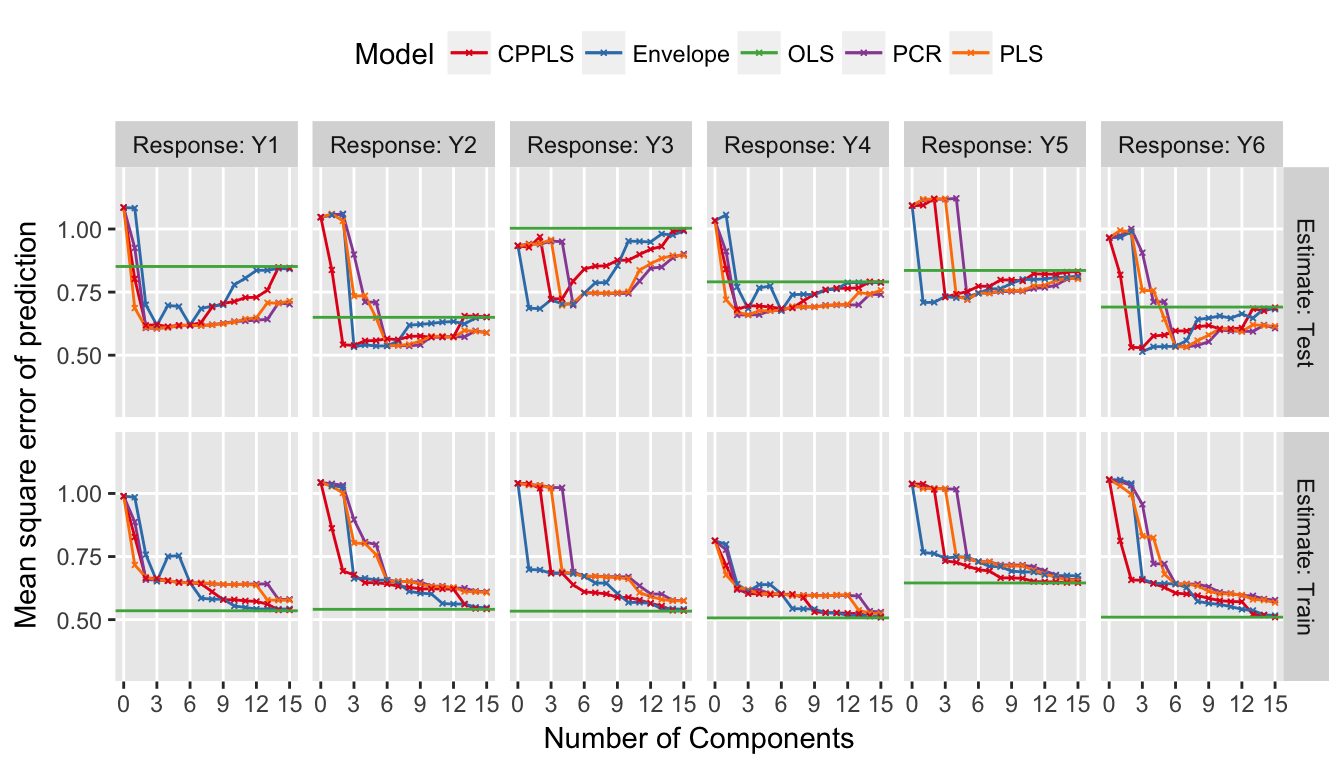
\includegraphics{Simrel-M_files/figure-latex/pred-plot-1-1.pdf}
\caption{\label{fig:pred-plot-1}Model comparison based on prediction error
for each response.}
\end{figure}

\begin{figure}
\centering
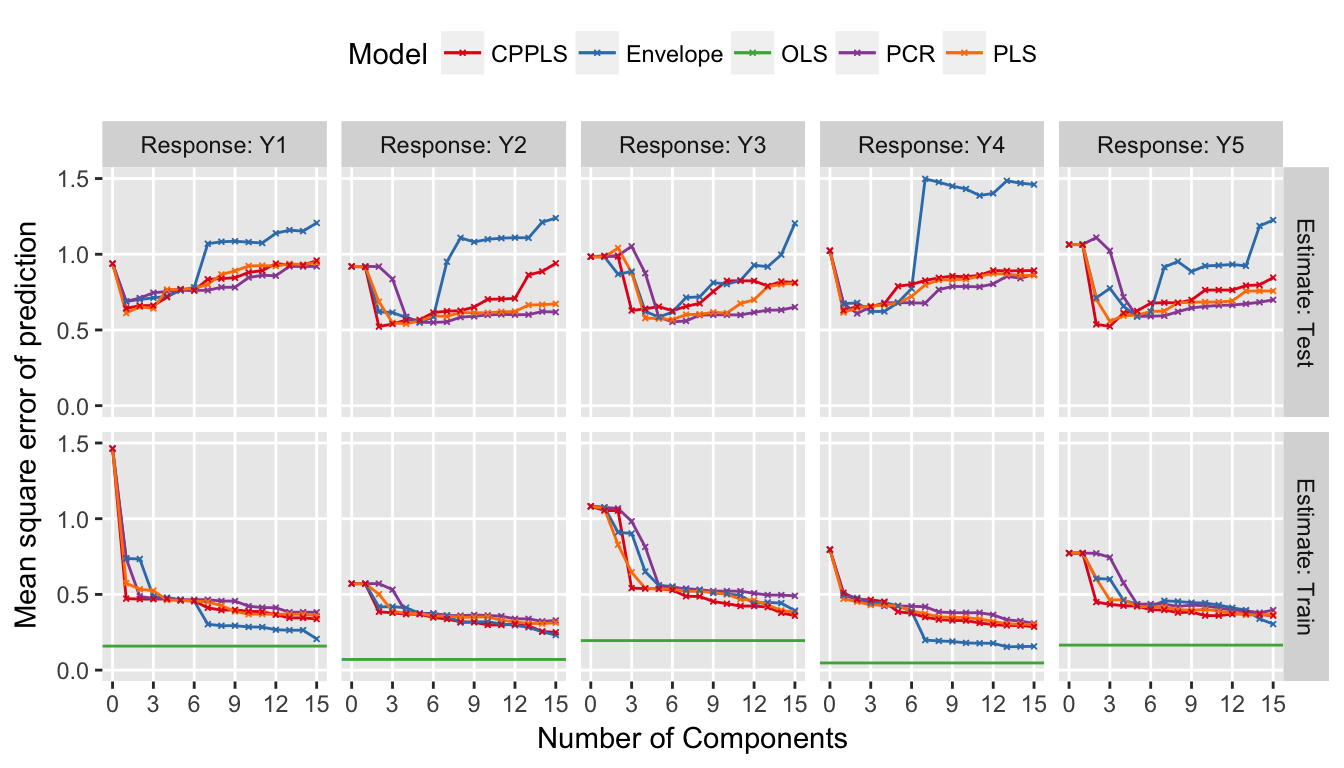
\includegraphics{Simrel-M_files/figure-latex/pred-plot-2-1.pdf}
\caption{\label{fig:pred-plot-2}Train and test prediction error for
different response comparing models under comparison}
\end{figure}

\renewcommand\refname{References}
\bibliography{packages.bib,ref-db.bib}

\end{document}
